\documentclass{article}
\usepackage[a4paper, margin=2.5cm]{geometry}
\usepackage{amsmath}
\usepackage{amssymb}
\usepackage{mathtools}
\usepackage{enumitem}
\usepackage{graphicx}
\usepackage{booktabs}
\usepackage{microtype}
\usepackage[parfill]{parskip}
\usepackage{xcolor}
\usepackage{listings}
\usepackage{hyperref}

\lstset{
    basicstyle=\ttfamily\small,
    keywordstyle=\color{blue},
    commentstyle=\color{gray},
    stringstyle=\color{teal},
    showstringspaces=false,
    breaklines=true,
    frame=single
}

\title{Cybersecurity Risk Homework 2B}
\author{Philipp Zhuravlev}
\date{3 October 2026}

\begin{document}

\maketitle

\section*{Part 1}

The first vulnerability is a classic SQL injection in the user field, which comments out anything past \texttt{--} and returns the first user, the admin:

\begin{center}
    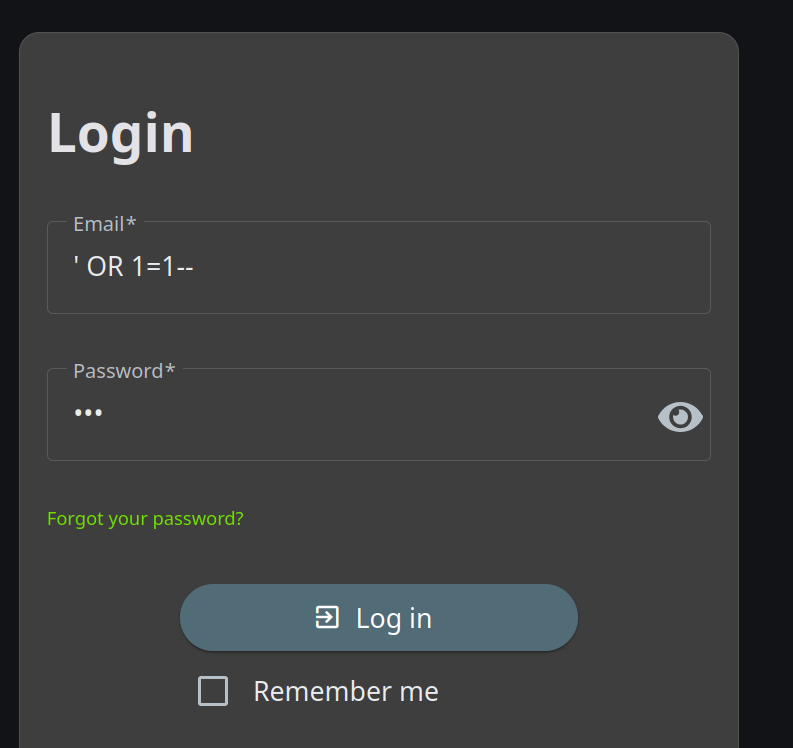
\includegraphics[width=0.39\textwidth]{Screenshots/001.png}
    \hfill
    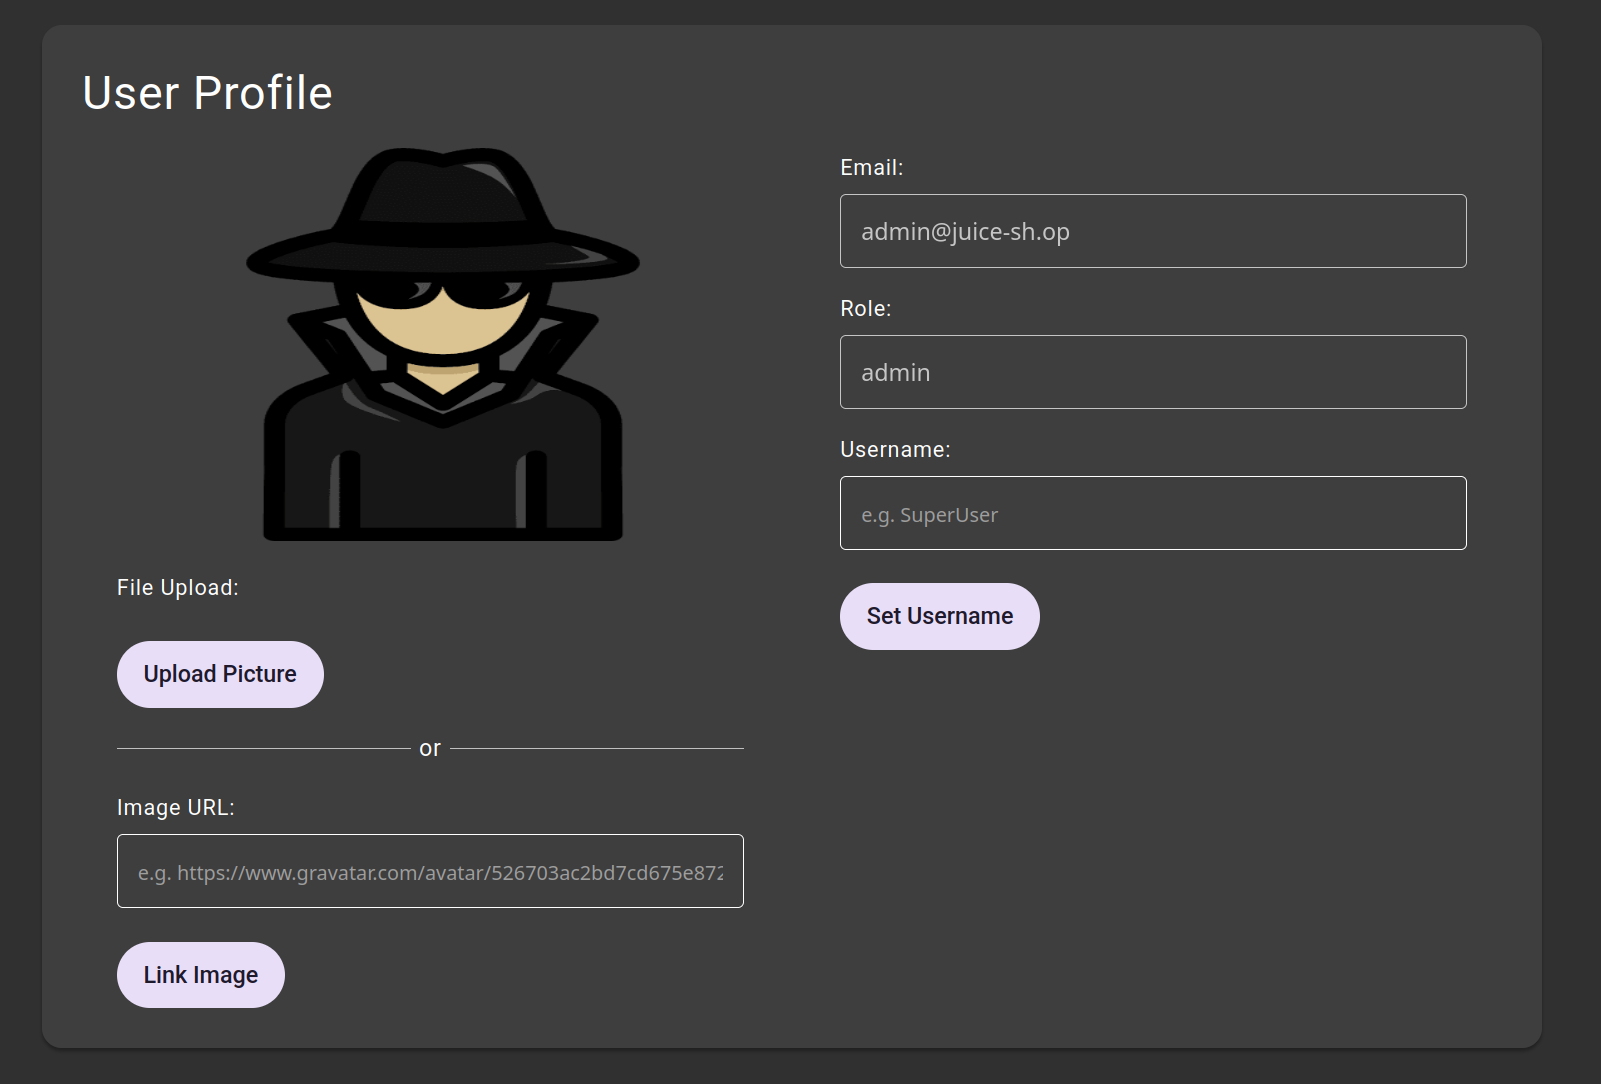
\includegraphics[width=0.53\textwidth]{Screenshots/002.png}
\end{center}

To fix this, queries need to be parameterized so input is treated as data, not SQL. Next, I showed the website is vulnerable to XSS, meaning I can execute code on it:

\begin{center}
    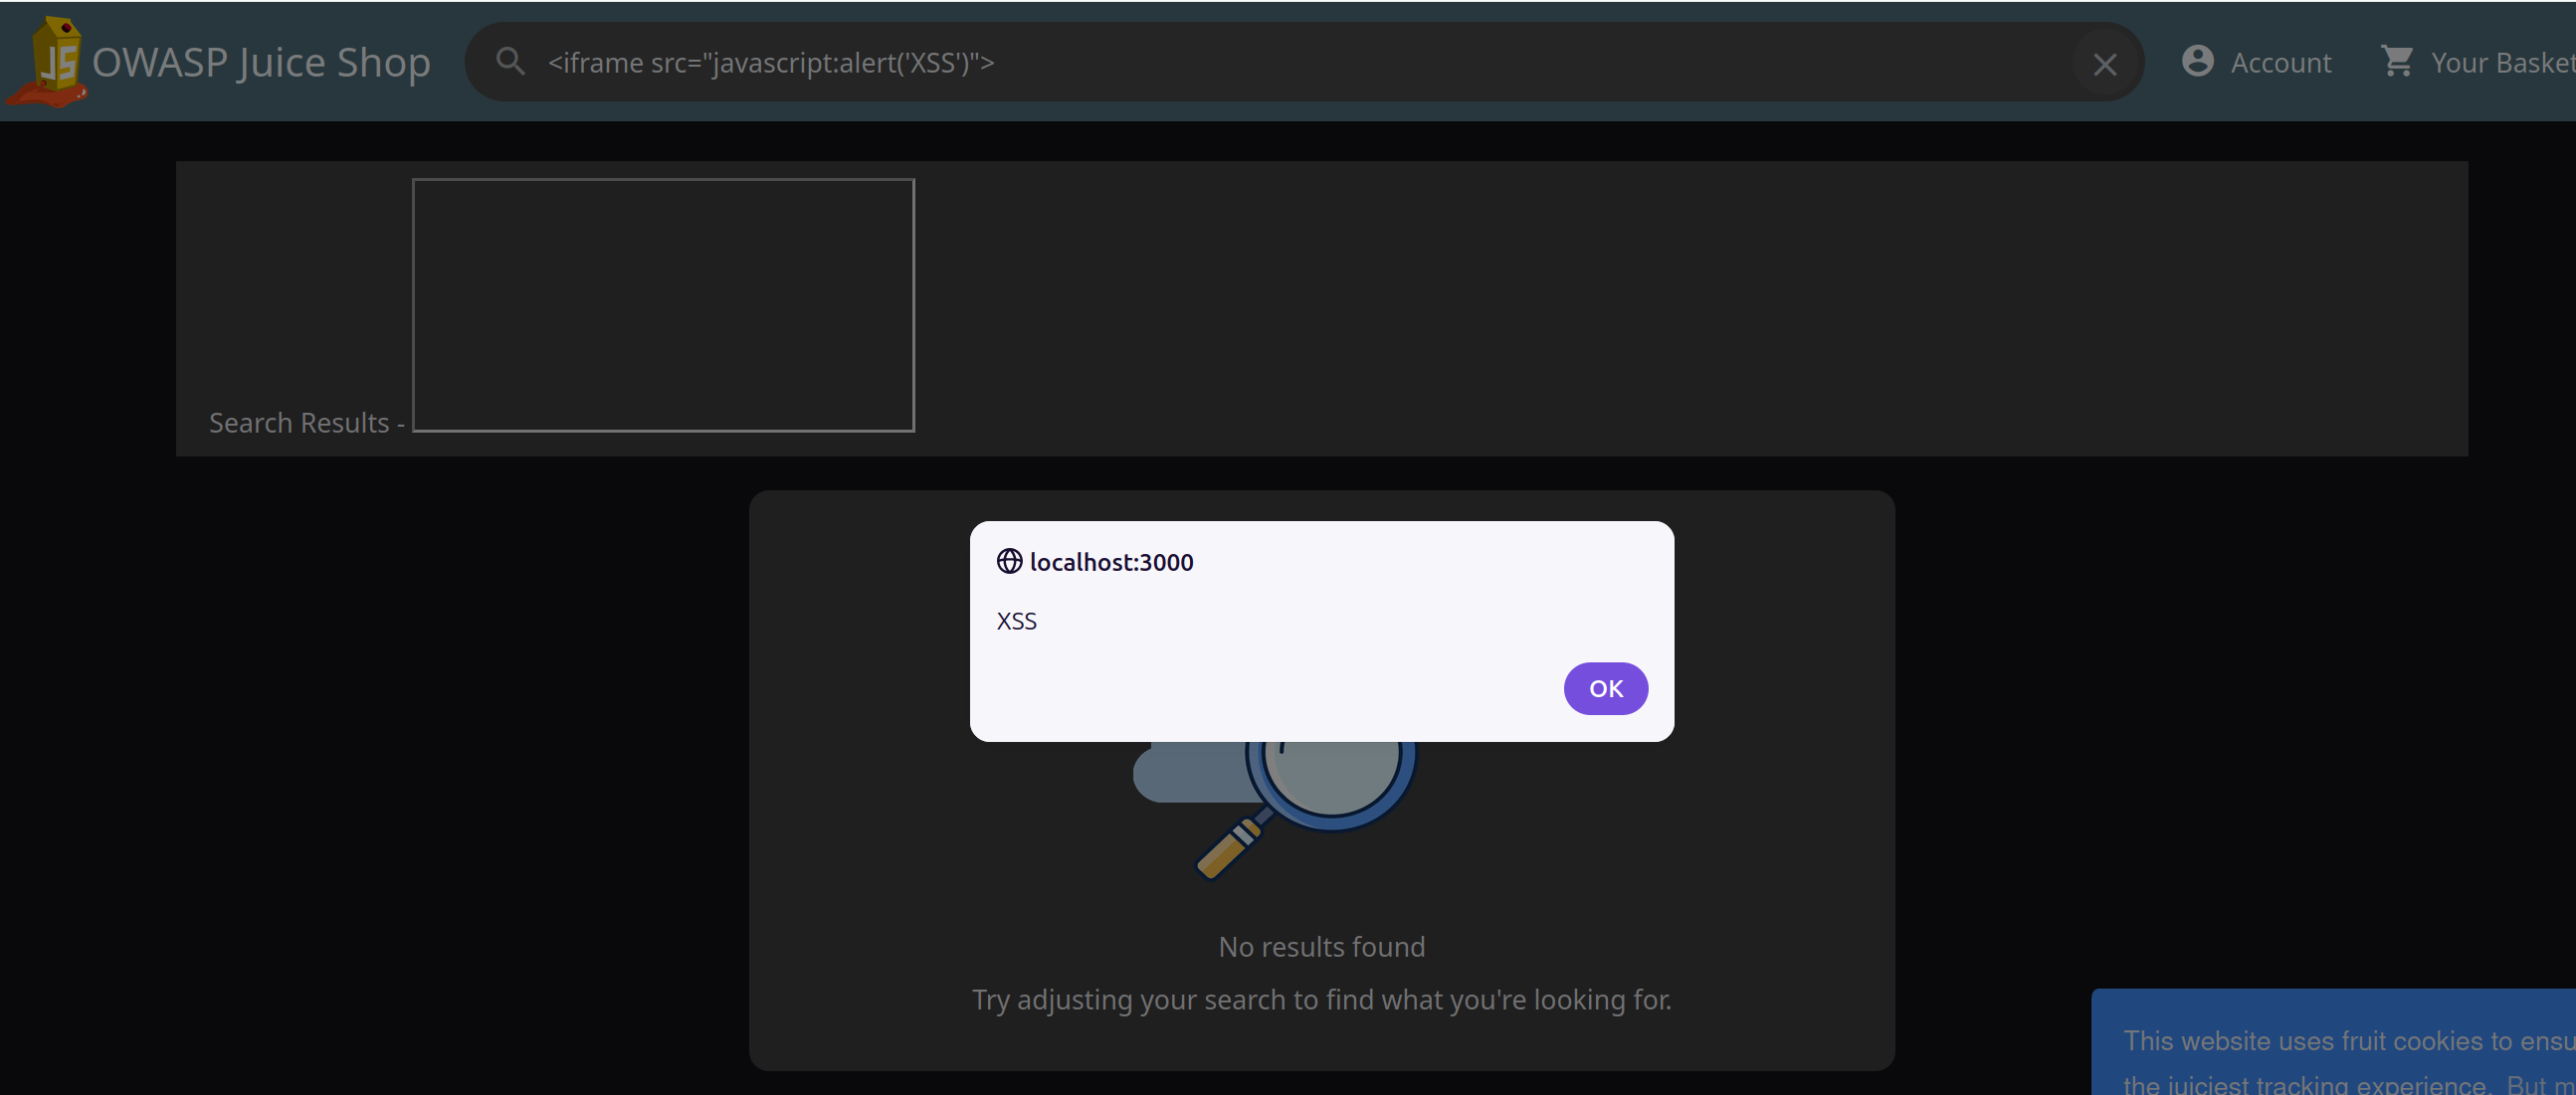
\includegraphics[width=0.6\textwidth]{Screenshots/003.png}
\end{center}

A fix is output encoding, so tags show as text, and CSP to block inline scripts. Lastly, a POST to \texttt{/api/Users} with \texttt{"role": "admin"} in the body created an admin account:

\begin{center}
    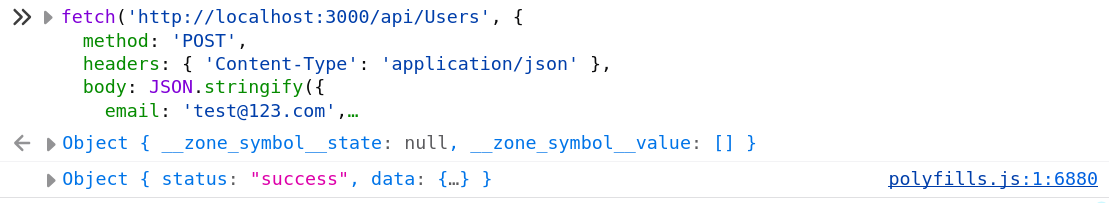
\includegraphics[width=0.6\textwidth]{Screenshots/004.png}
\end{center}

The fix is a server-side allow-list that drops fields like \texttt{role}. Passwords should be hashed with bcrypt so a leak doesn't expose them:

\begin{lstlisting}
const hash = bcrypt.hashSync(password, 10);    // on register
const ok = bcrypt.compareSync(password, hash); // on login
\end{lstlisting}

\section*{Part 2}

I built a simple login form with HTML and JS, using a small Express server over Node, hosting a SQLite DB. The form just has email and password, where the client has basic validation (not empty, contains @, password at least 8 chars) before being sent. The server does the same checks to prevent the same type of client-side bypasses as above. The DB only has a Users table, storing parameterized queries to prevent SQL injection like above; passwords are also hashed with bcrypt. Messages are shown with \texttt{textContent} instead of \texttt{innerHTML}, so injected HTML displays as plain text.

\medskip
GitHub: \url{https://github.com/philip-crane/HW-2B}

\section*{Part 3}

I tried to break my own form three ways. First, SQL injection with \texttt{x@x' OR 1=1 --}, which includes a @ so it isn't rejected by the email validation. It still fails, since the parameterized query treats it as plain text instead of SQL:

\begin{center}
    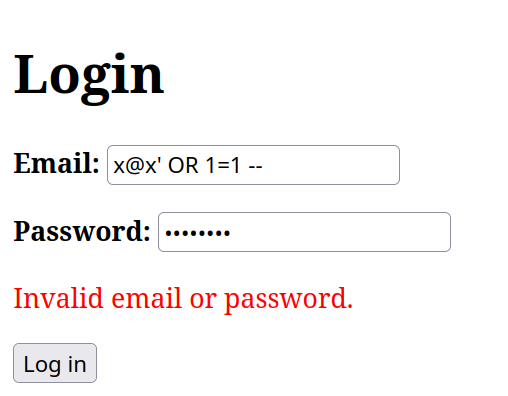
\includegraphics[width=0.40\textwidth]{Screenshots/005.png}
\end{center}

Next I attempted an XSS attack through the console, setting \texttt{textContent} to the img onerror payload the same way my app does. The script doesn't run, and just displays as inert text:

\begin{center}
    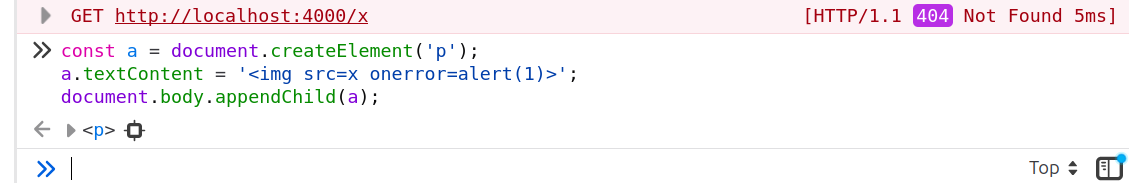
\includegraphics[width=0.9\textwidth]{Screenshots/006.png}
\end{center}

Lastly, since client-side checks can be skipped, I called the API directly with an invalid email. The server validates again and rejects it:

\begin{center}
    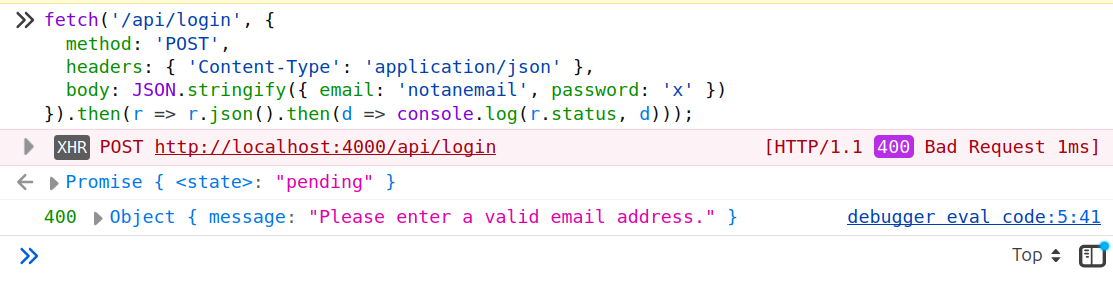
\includegraphics[width=0.9\textwidth]{Screenshots/007.png}
\end{center}

None worked. Adding a CSP header would harden it further.

\end{document}
